\documentclass{article}

\usepackage{graphicx}


\begin{document}

Questions on trigonometry from the aptitude test organized at Ghent University in various years. \LaTeX expressions can directly be pasted into Wooclap.

\section{}

Suppose $\displaystyle\sin(x) = \frac{2}{3}$, with $\frac{\pi}{2} < x < \pi$. Find the value of $\sin(2x)$.

\begin{enumerate}
\item $\displaystyle\frac{-4\sqrt{5}}{9}$ %
\item $\displaystyle\frac{-\sqrt{5}}{3}$
\item $\displaystyle\frac{\sqrt{5}}{3}$
\item $\displaystyle\frac{4\sqrt{5}}{9}$
\end{enumerate}

\section{}
Consider the right-angled triangle $ABC$ as shown on the figure. You know that the length of sides are given by $|AB| = 5$ and $|BC| = 13$. What is the value of the height $h$ of the triangle?

\includegraphics{./images/triangle.png}

\begin{enumerate}
\item $3$
\item $4$
\item $\displaystyle\frac{48}{13}$
\item $\displaystyle\frac{60}{30}$ %
\end{enumerate}

\section{}

You know that $\displaystyle \sin x \left( \tan x + \frac{1}{\tan x} \right) = 2$. Which of the following expressions is true?
\begin{enumerate}
\item $\displaystyle\frac{1}{\cos x} = 2$
\item $\displaystyle\frac{1}{\sin x} = 2$
\item $\displaystyle\frac{1}{\tan x} = 2$
\item $\displaystyle\tan x  = 2$
\end{enumerate}

\end{document}
